\documentclass[aps,prl,reprint,amsmath,amssymb,superscriptaddress]{revtex4-2}

% ── Packages ─────────────────────────────────────────────────────────────────
\usepackage{graphicx}          % external figures (PNG, PDF)
\usepackage{hyperref}          % clickable references and DOI links
\usepackage{siunitx}           % consistent units: \qty{3.5}{\angstrom}
\usepackage{cleveref}          % \cref{fig:band} → "Fig. 1"
\usepackage{booktabs}          % publication-quality tables
\usepackage{xcolor}            % colour for todo notes
\usepackage[normalem]{ulem}    % \sout for strikethrough in revision

% ── Native LaTeX plotting ─────────────────────────────────────────────────────
\usepackage{pgfplots}
\pgfplotsset{compat=1.18}

% ── Custom units (siunitx) ────────────────────────────────────────────────────
\DeclareSIUnit{\atom}{atom}
\DeclareSIUnit{\formulaunit}{f.u.}

% ── Placeholder & revision helpers (remove before submission)
\usepackage{lipsum}           % lorem ipsum: \lipsum[1-3] — delete when writing
\newcommand{\todo}[1]{\textcolor{red}{\textbf{[TODO: #1]}}}
\newcommand{\note}[1]{\textcolor{blue}{\textit{[#1]}}}

% ─────────────────────────────────────────────────────────────────────────────
\begin{document}

\title{Paper Title}

\author{First Author}
\affiliation{Department of Chemistry and Bioscience,
             Aalborg University, DK-9220 Aalborg, Denmark}

\author{Second Author}
\affiliation{Department of Chemistry and Bioscience,
             Aalborg University, DK-9220 Aalborg, Denmark}

\author{Third Author}
\email{email@bio.aau.dk}
\affiliation{Department of Chemistry and Bioscience,
             Aalborg University, DK-9220 Aalborg, Denmark}

\date{\today}

% ─────────────────────────────────────────────────────────────────────────────
\begin{abstract}
\lipsum[1][1-6]

\end{abstract}

\maketitle

% ─────────────────────────────────────────────────────────────────────────────
\section{Introduction}

\lipsum[1-3]
\section{Methods}
\label{sec:methods}

\subsection{Computational Details}

All calculations were performed using \todo{code name}~\cite{placeholder2024}
within the generalized gradient approximation (GGA) as parametrized by
Perdew, Burke, and Ernzerhof (PBE)~\cite{placeholder2024}.
Structures were relaxed until forces fell below
\qty{0.01}{\electronvolt\per\angstrom}.

\lipsum[4-5]

\section{Results and Discussion}
\label{sec:results}

\subsection{Convergence}

\lipsum[6]

% ── PNG figure (exported from a Python/matplotlib script in figures/) ─────────
\begin{figure}
  \centering
  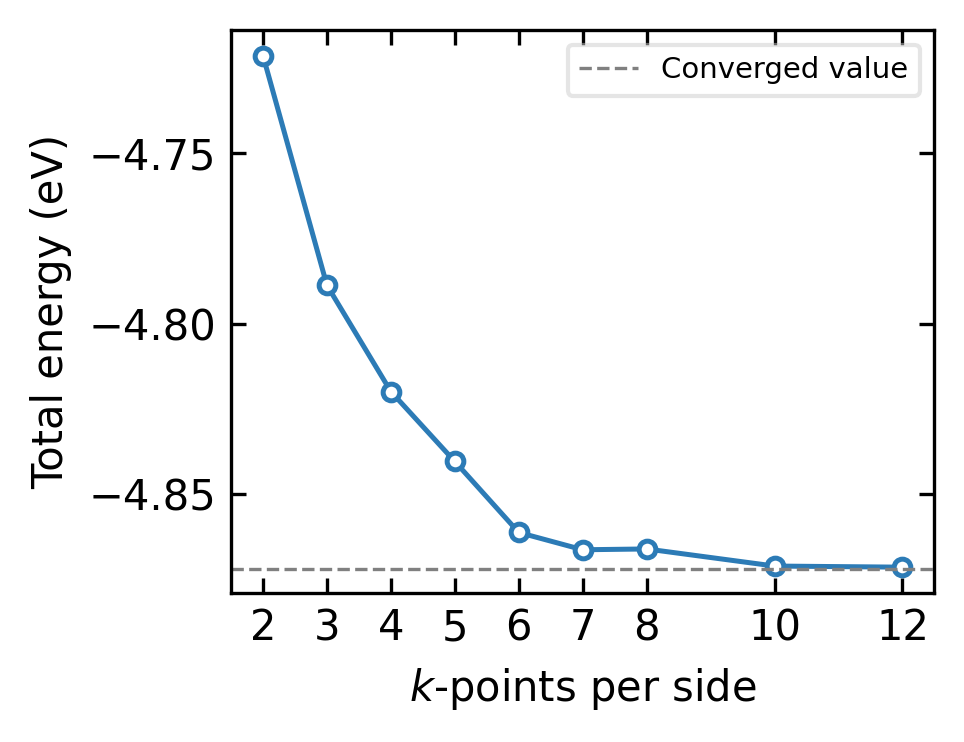
\includegraphics[width=\columnwidth]{figures/kpoint-convergence.png}
  \caption{%
    \textbf{$k$-point convergence.}
    Total energy as a function of $k$-points per side of the
    Monkhorst–Pack mesh.
    The dashed line marks the value used in all subsequent calculations.
  }
  \label{fig:kconv}
\end{figure}

\subsection{Main result}

\lipsum[7]

% ── pgfplots figure (data embedded directly — good for small datasets) ────────
\begin{figure}
  \centering
  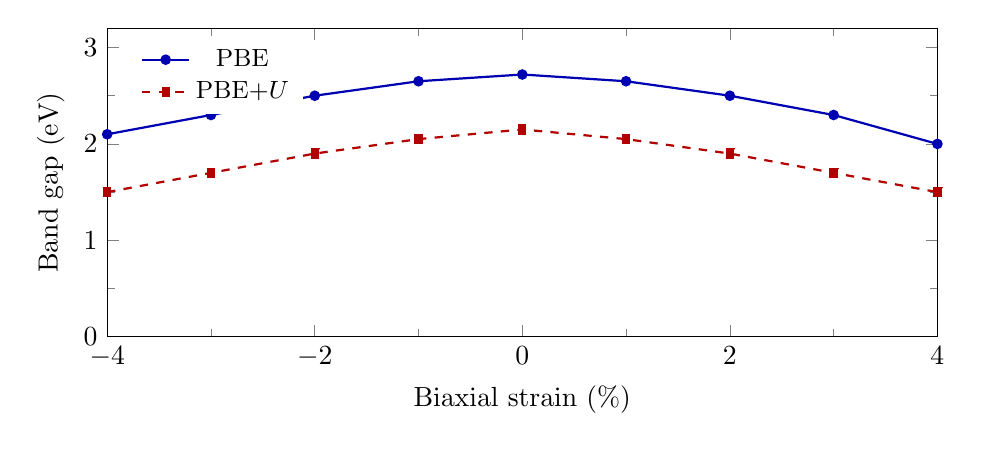
\begin{tikzpicture}
    \begin{axis}[
      width  = \columnwidth,
      height = 5.5cm,
      xlabel = {Biaxial strain (\%)},
      ylabel = {Band gap (eV)},
      xmin = -4, xmax = 4,
      ymin =  0, ymax = 3.2,
      xtick distance = 2,
      minor tick num  = 1,
      tick align = inside,
      axis line style = {thin},
      legend pos = north west,
      legend style = {font=\small, draw=none},
    ]
      \addplot[thick, color=blue!70!black, mark=*, mark size=1.5pt]
        coordinates {(-4,2.1)(-3,2.3)(-2,2.5)(-1,2.65)(0,2.72)(1,2.65)(2,2.5)(3,2.3)(4,2.0)};
      \addlegendentry{PBE}

      \addplot[thick, dashed, color=red!70!black, mark=square*, mark size=1.5pt]
        coordinates {(-4,1.5)(-3,1.7)(-2,1.9)(-1,2.05)(0,2.15)(1,2.05)(2,1.9)(3,1.7)(4,1.5)};
      \addlegendentry{PBE+$U$}
    \end{axis}
  \end{tikzpicture}
  \caption{%
    \textbf{Strain-tunable band gap.}
    Fundamental band gap as a function of biaxial strain.
    \todo{Replace with real data.}
  }
  \label{fig:pgf}
\end{figure}

\lipsum[8]

\section{Conclusion}
\label{sec:conclusion}

\lipsum[9]


% ─────────────────────────────────────────────────────────────────────────────
\begin{acknowledgments}
The authors acknowledge compute time on \todo{cluster name}.
\end{acknowledgments}

\bibliography{references}

\end{document}
